\section{Evaluation}
\label{sec:eval}

\subsection{Micro-Benchmark Results}
\label{sec:sims}

\begin{enumerate}
    \item CDF of Average Decoding Time (Genie)
    \begin{enumerate}
        \item The first re-transmission is the most critical for small to moderate size packets because MAC overhead is still significant.
        \item For large packet sizes, MAC overhead is almost negligible, hence, it is worth re-transmitting a second time.
    \end{enumerate}


\begin{figure}[t]
\centering
\vspace*{-0.1in}
\subfigure[CDF of Average Decoding Time] {
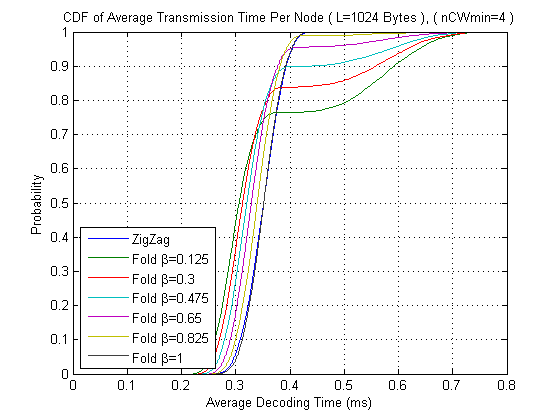
\includegraphics[width=.9\columnwidth]{./figs/cdf_1024_ht_all_qam.png}
\label{fig:cdf_avg_1024}
}
\vskip -0.5em
\caption{CDF of Average Decoding Time (L=1024)}
%\vskip -1em
\end{figure}

\begin{figure}[t]
\centering
\vspace*{-0.1in}
\subfigure[CDF of Average Decoding Time] {
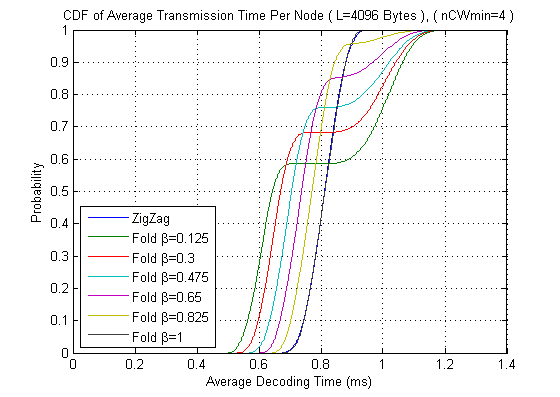
\includegraphics[width=.9\columnwidth]{./figs/cdf_4096_ht_all_qam.png}
\label{fig:cdf_avg_4096}
}
\vskip -0.5em
\caption{CDF of Average Decoding Time (L=4096)}
%\vskip -1em
\end{figure}

\end{enumerate}

%%\subsection{Experimental Results}
%%\label{sec:experimental}

%%1. Packet Reception Ratio / Bit-Error-Rate
%%(a) Standard
%%(b) RoXOR
%%(c) ZigZag?

%%2. CDF of Average Decode Time
%%(a) Standard
%%(b) RoXOR
%%(c) ZigZag?


